\documentclass[journal, a4paper,onecolumn]{IEEEtran}
\IEEEoverridecommandlockouts
\usepackage{cite}
\usepackage{amsmath,amssymb,amsfonts}
\usepackage{algorithmic}
\usepackage{graphicx}
\usepackage{textcomp}
\usepackage{xcolor}
\usepackage{parskip}
\usepackage{hyperref}
\usepackage{booktabs}
\usepackage[super]{nth}
\usepackage{colortbl}
\usepackage{lipsum}  
\usepackage{subcaption}

\def\BibTeX{{\rm B\kern-.05em{\sc i\kern-.025em b}\kern-.08em
    T\kern-.1667em\lower.7ex\hbox{E}\kern-.125emX}}

\def\thesubsubsectiondis{\thesubsectiondis\arabic{subsubsection}}

\makeatletter
\def\subsubsection{%
  \@startsection
    {subsubsection}                 % type
    {3}                             % level
    {\parindent}                    % indent
    {3.5ex plus 1.5ex minus 1.5ex}  % beforeskip {0ex plus 0.1ex minus 0.1ex}
    {0.7ex plus .5ex minus 0ex}     % afterskip {0ex}
    {\normalfont\normalsize\itshape}% style
}
\makeatother


\begin{document}

\title{\fontsize{20}{19.2}\selectfont Report Title}

\author{\IEEEauthorblockN{Student Number\\University of The Witwatersrand
\\School of Electrical and Information Engineering\\Course Code}
\IEEEauthorblockA{\\
Date\\}
}

\maketitle
\thispagestyle{plain}
\pagestyle{plain}

\begin{abstract}
\lipsum[1]
\end{abstract}

\begin{IEEEkeywords}
Lorum, ipsum, sit
\end{IEEEkeywords}
\section{Introduction}
\lipsum[2-3] \cite{b1}
\begin{thebibliography}{00}
\bibitem{b1} “Play original defender game online - arcade, Nintendo, Atari and Sega Games,” Free80sArcade, https://www.free80sarcade.com/defender.php (accessed Month. Day, Year). 
\end{thebibliography}

\clearpage  
\onecolumn
\appendices

\section{Figures}
\label{FiguresAppendix}

\begin{figure}[hbp]
  \centering
  \captionsetup{justification=centering}
  \centerline{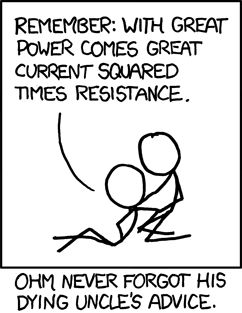
\includegraphics[width=0.5\linewidth]{Figures/fig1.jpg}}
  \caption{Class Diagram Illustrating Inter-Class Functionality and Inheritance}
  \label{inheritanceDiagram}
\end{figure}

\section{Tables}
\label{TablesAppendix}

\begin{table}[htbp]
\caption{An Example of a Table}
\begin{center}
\begin{tabular}{|ll|}
\hline
\multicolumn{2}{|c|}{\textbf{Features Implemented}}     \\ \hline
\multicolumn{1}{|l|}{\textbf{Major}} & \textbf{Minor}   \\ \hline
\multicolumn{1}{|l|}{Humanoids}      & Scoring system   \\ \hline
\end{tabular}
\label{tblFeatures}
\end{center}
\end{table}


\end{document}
